\documentclass[12pt,a4paper]{article}
\usepackage[utf8]{inputenc}
\usepackage[spanish]{babel}
\usepackage{amsmath}
\usepackage{amsfonts}
\usepackage{amssymb}
\usepackage{graphicx}
\usepackage[left=2cm,right=2cm,top=2cm,bottom=2cm]{geometry}
\author{Enciso Guerrero Benjamin Salvador\\
Carlos Enrrique Moran Garabito\\
Cinematica De Robots }
\title{Condiciones de Singularidades de manipuladores.}
\begin{document}
\maketitle

\includegraphics[scale=1.8]{upzmgg.jpg} 
\newpage
Condiciones de Singularidades de manipuladores.
\\\\
Se dice que un manipulador tiene (n) grados de libertad (GdL) si su configuración puede ser especificada, como mínimo, por (n) variables independientes. Por lo tanto, la dimensión de C es igual al número de GdL. Para un manipulador serie, el número de articulaciones simples determina el número de GdL. Para la tarea de posicionar y orientar el elemento terminal en el espacio cartesiano se requiere un mínimo de 6 GdL, por lo que los robots con más de 6 GdL se denominan redundantes para esta tarea mientras que el resto se denominan no-redundantes. 
\\\\
El estudio de los diversos problemas cinemáticos tiene gran importancia debido a su trascendencia en la manipulación y control de los robots. Especialmente importantes son los problemas relacionados con las singularidades y la cinemática inversa. 
\\\\
Las singularidades son aquellas configuraciones que limitan el movimiento del robot manipulador debido a que: 
\\\\
a) Corresponden a configuraciones desde/hacia las que el elemento terminal no puede trasladarse o rotar en alguna o algunas direcciones del espacio. 
\\\\
b) Representan configuraciones en las que se requieren velocidades articulares no acotadas para obtener velocidades finitas del elemento terminal.
\\\\
Por otro lado, la resolución de la cinemática inversa de los robots manipuladores serie consiste en obtener las configuraciones asociadas a una pose concreta del elemento terminal. Las soluciones de la cinemática inversa se clasifican en dos grupos:
\\\\
*Soluciones analíticas o en forma cerrada: Se obtienen todas las soluciones, que se describen mediante funciones analíticas.
\\\\
*Soluciones numéricas: Se obtiene una única buena aproximación de una de las configuraciones solución mediante un algoritmo iterativo. Para manipuladores redundantes, existen algoritmos que, usando el espacio nulo del jacobiano, resuelven tareas secundarias como evitar singularidades, evitar limites articulares, etc. 
\\\\
Singularidades: 
\\\\Una singularidad es aquella configuración en la que el manipulador pierde algunos de sus grados de libertad. Esto se traduce en que el elemento terminal pierde la capacidad de movimiento en ciertas direcciones y en que se requieren velocidades articulares infinitas para generar velocidades lineales y angulares finitas del elemento terminal. (Hollerbach, 1985; Gottlieb, 1986) 
\\\\
demuestran de forma independiente que cualquier manipulador serie de n > 2 GdL posee singularidades. 
\\\\
Para robots manipuladores redundantes, las singularidades pueden obtenerse mediante dos enfoques diferentes: 
\\\\
C1: Resolviendo una ecuación no lineal. Esta forma es más compleja de abordar sin usar métodos numéricos, pero es la más general. 
\\\\
C2: Para aquellos manipuladores redundantes con muñeca esférica, las singularidades pueden desacoplarse en: singularidades de posicion, orientación y acopladas. Para ello se consideran las submatrices del jacobiano (2). 
\\\\
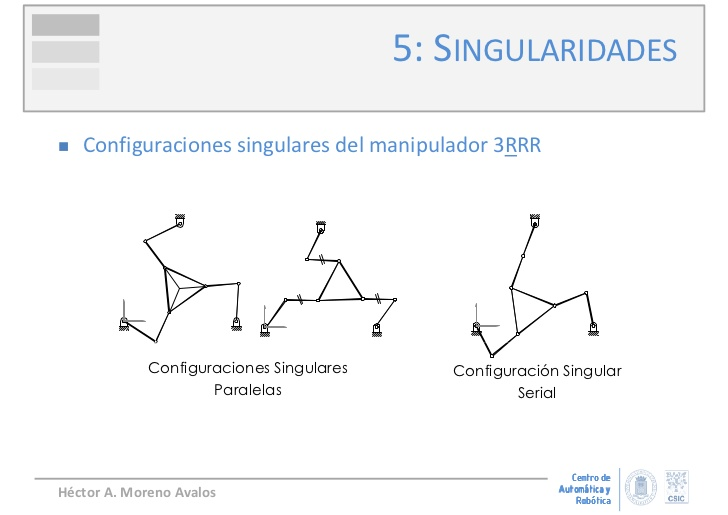
\includegraphics[scale=0.6]{robots-paralelos-conceptos-y-aplicaciones-22-728.jpg} 
\\
figura1.singularidades paralelas y seriales.
\\\\
Se llama singularidad limite cuando el manipulador está completamente distendido o retraído. 
\\\\
Se llama singularidad interna cuando ocurre el alineamiento de dos o más ejes de los sistemas de coordenadas, tornando las líneas del Jacobiano linealmente dependientes.
\\\\\\
Este tipo de singularidad puede ocurrir en cualquier posición del actuador final. 
\\\\
Es importante conocer las configuraciones singulares del robot por las siguientes razones: 
\\\\
Causa pérdida de movilidad del robot Cuando el robot está en una configuración singular, pueden existir infinitas soluciones para la cinemática inversa.
\\\\
Cuando el manipulador se aproxima a una configuración singular, una pequeña velocidad del actuador final provoca grandes velocidades en el accionamiento del robot.



\end{document}